\chapter{Konzept}

\label{ReportKonzept}

Durch die in der Studie gewonnenen Erkentnissen, werden in der Phase Konzept
verschiedene Teilkonzepte erstellt.

Im Teilkonzept «Portalname» wird der Name des Produktes erarbeitet.

Im Teilkonzept «Design- und Bedienkonzept» werden die Ansichten der Applikation
in Mockups umgesetzt. Es werden die Benutzer Use-Cases vom Besucher sowie der
Konzert-Erfasser aufgezeigt.

Im Teilkonzept «Softwarekonzept» werden die Datenflüsse hinter den Mockups
aufgezeigt, sowie die Datenbankstruktur aufgebaut.

Im Teilkonzept «Testkonzept» werden die einzelnen Systemtests aufgelistet sowie
ausgearbeitet wie granular welche Teile der Software getestet werden sollen.

Im letzten Teil des Konzept-Dokuments wird im Fazit dokumentiert, wie und warum
das Konzept von den vorhergehenden Phasen des Projekts abweicht.


\section{Portalname}\label{portalname}

Der Portalname wurde in einer Brainstorming-Session von Damian Senn auf
den Namen \textbf{«Gigpillar»} festgelegt. Der Name ist angelehnt an die Werbepfeiler in
Städten, wo oft Werbeplakate für Konzerte hängen.

Im Konzept im Anhang~\ref{portalname} ist eine Liste von Ideen für alternative Namen zu finden.

\clearpage
\section{Design}

\subsubsection{Homepage}

Die Homepage ist die erste Seite, die der Besucher sieht, wenn er/sie die
Applikation direkt über \href{https://gigpillar.com/}{gigpillar.com} aufruft.
Auf den ersten Blick ist die Suche sowie ein grosses Bild (Banner) eines Gigs
zu erblicken. Weiter sind Links zu gängigen Funktionalitäten wie Gig hinzufügen
sowie das Login in einer Navigation erreichbar.

Unter dem Banner werden Gigs in nächster nähe des Besuchers aufgelistet, der
Link «change location» führt weiter zur Suchresultate Seite um den
entsprechenden Filter anzupassen.

\begin{figure}[!htb]
  \centering
  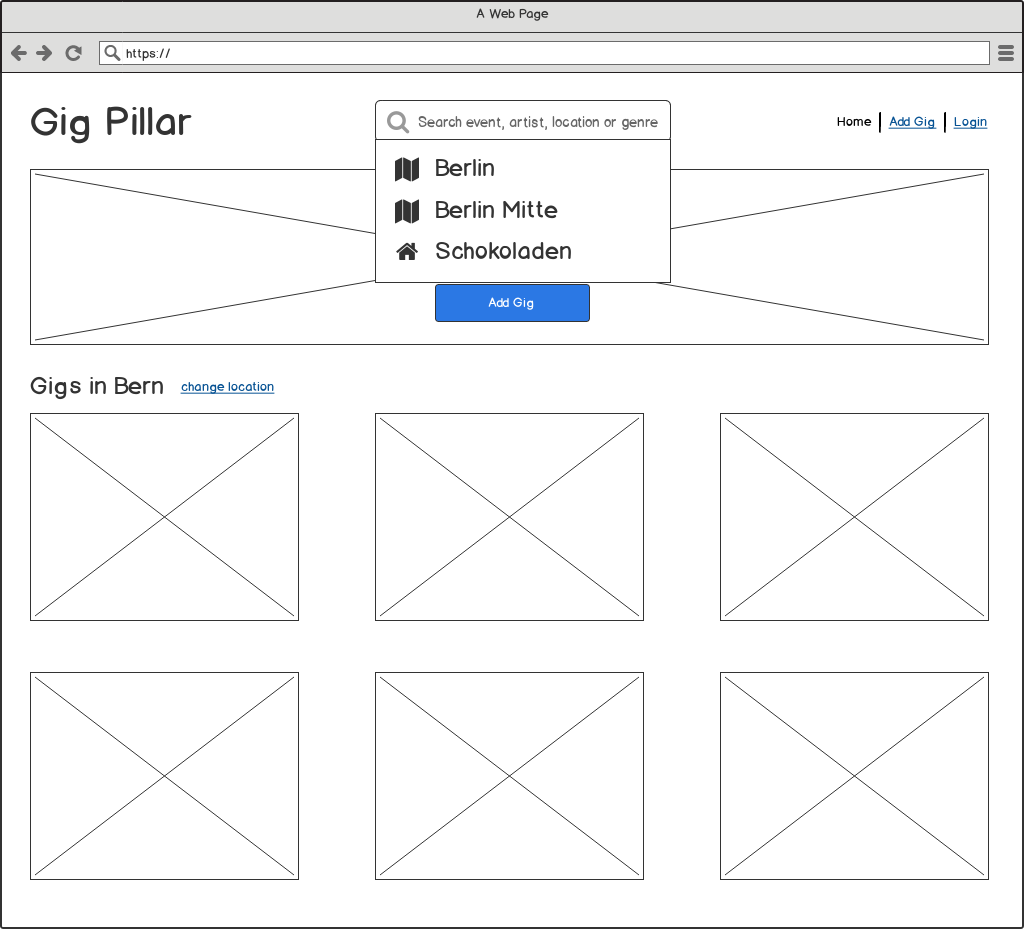
\includegraphics[width=0.95\textwidth]{mockups/homepage.png}
  \caption{Mockup: Homepage}
\end{figure}

\clearpage
\subsubsection{Suchresultate}

Auf der Suchresultate Seite sieht der Benutzer seine Suchresultate der von der
globalen Suchbox ausgelösten Suche. Die Seite bietet weitere Filter an um die
Resultate weiter einzugrenzen.\\

\noindent
Folgende Filter stehen den Benutzern zur Verfügung:

% TODO: This diverges from our search criteria described in the previous phase.

\begin{itemize}
  \tightlist{}
  \item{} Ort
  \item{} Datum von
  \item{} Datum bis
  \item{} Musik Genre
\end{itemize}

\noindent
Das Anwählen eines Suchresultates führt den Benutzer weiter zur detaillierten
Gig Ansicht.

\begin{figure}[!htb]
  \centering
  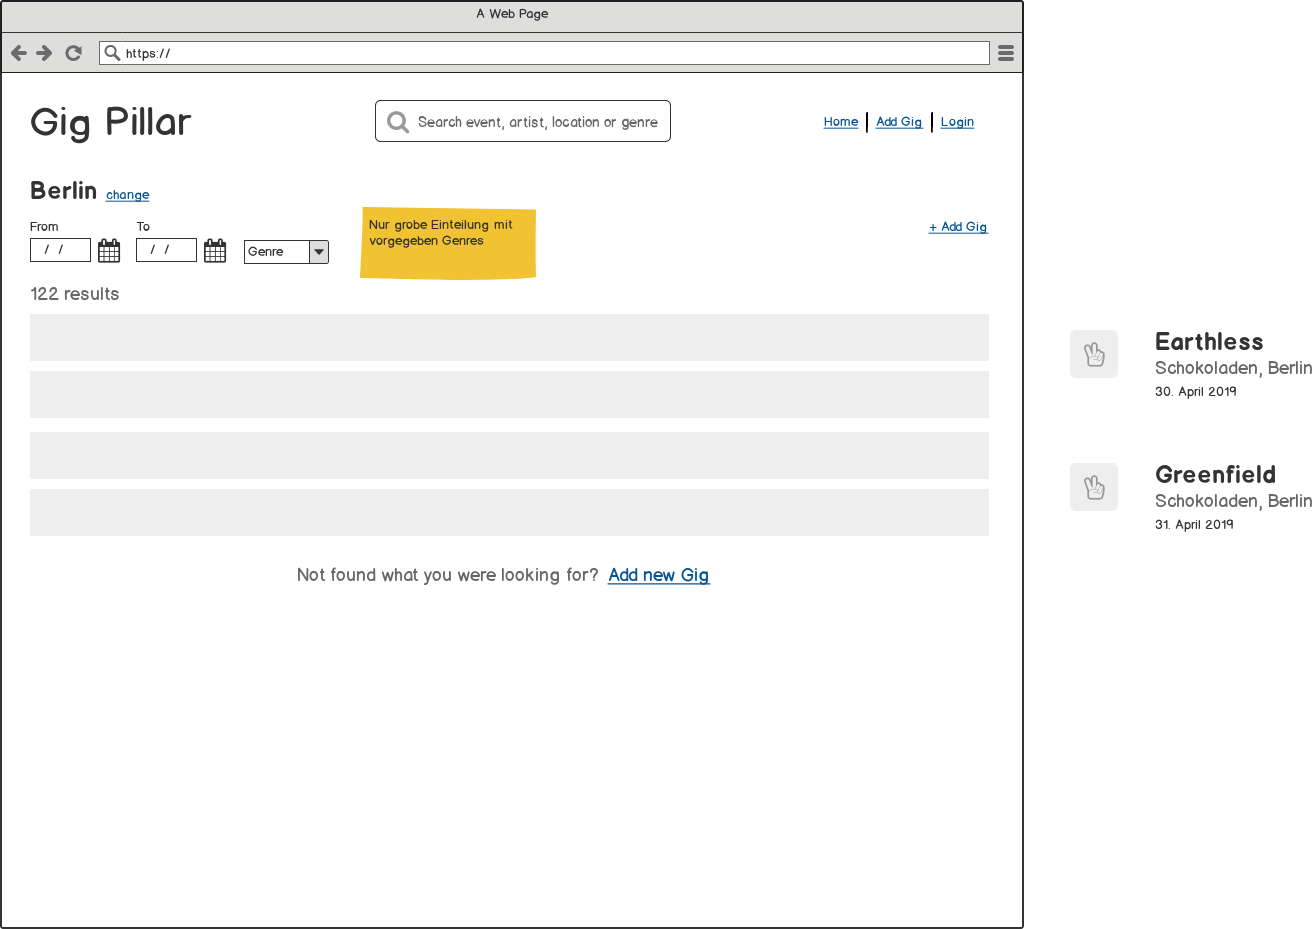
\includegraphics[width=0.95\textwidth]{mockups/search-result.png}
  \caption{Mockup: Suchresultate}
\end{figure}

\clearpage
\subsubsection{Gig Ansicht}

In der Gig Ansicht werden alle Details zu einem Event aufgelistet.

\begin{itemize}
  \tightlist{}
  \item{} Datum des Events
  \item{} Zeit wann das Event beginnt, bzw die Location die Türen öffnet
  \item{} Liste aller Künstler mit optionaler Startzeit
  \item{} Eine Beschreibung des Events
  \item{} Die Adresse der Location mit Link auf Google Maps
\end{itemize}

\noindent
Ausserdem soll es den Benutzern möglich sein, über einen «Add to my calendar»
Link das Event zu seiner Kalender-Applikation zu importieren.

\begin{figure}[!htb]
  \centering
  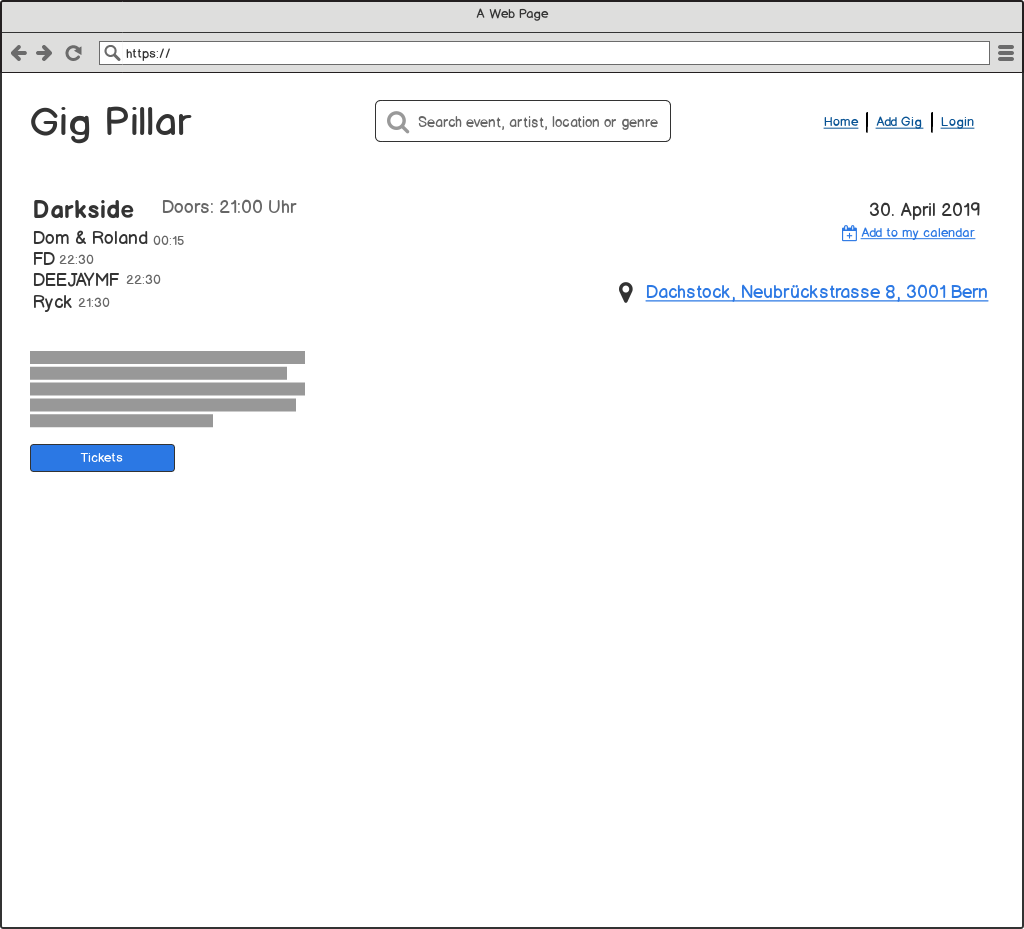
\includegraphics[width=0.95\textwidth]{mockups/event.png}
  \caption{Mockup: Gig Ansicht}
\end{figure}

\clearpage
\subsubsection{Gig erfassen}

Benutzer können Gigs erfassen.\\

\noindent
Folgende Daten sind für einen Gig zu erfassen:

\begin{itemize}
  \tightlist{}
  \item{} Name
  \item{} Bild \textit{(optional)}
  \item{} Location
  \item{} Datum
  \item{} Zeit
  \item{} Eine Liste von Artists mit optionaler Startzeit
  \item{} Beschreibung
  \item{} Link zum Ticketvertreiber
\end{itemize}

\begin{figure}[!htb]
  \centering
  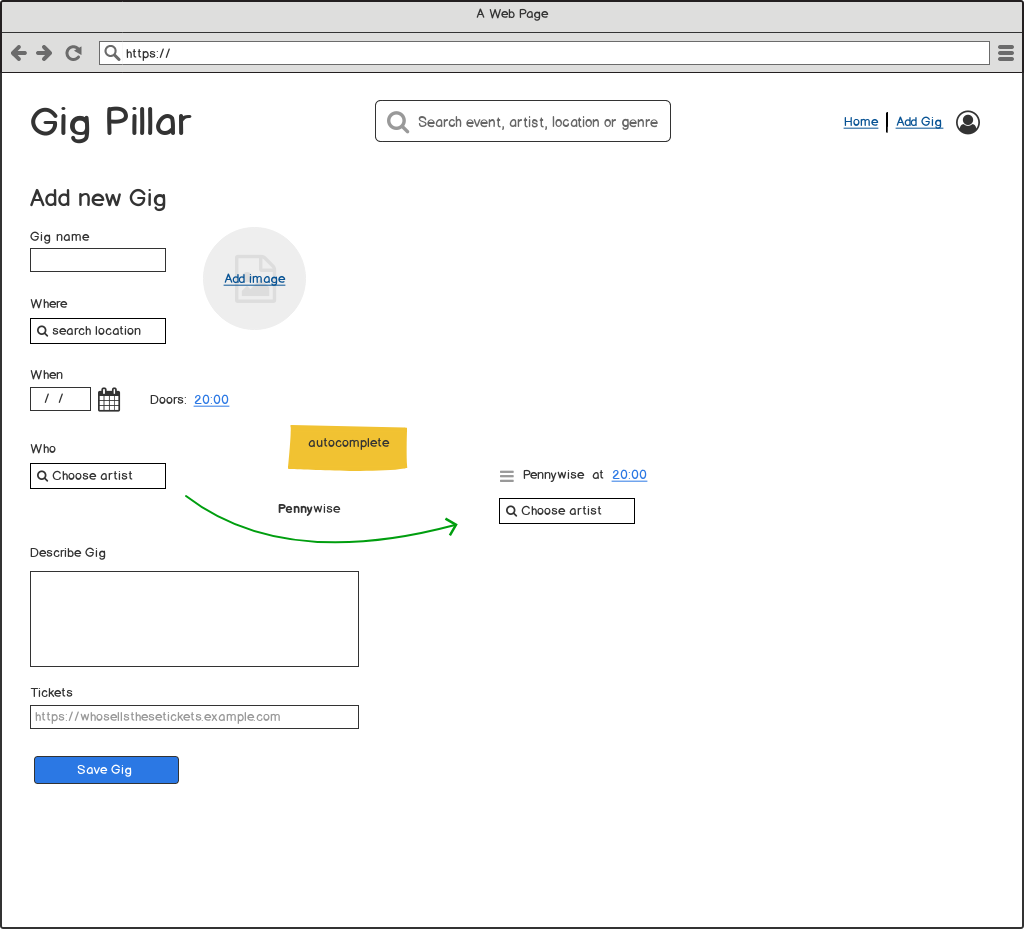
\includegraphics[width=0.95\textwidth]{mockups/add-gig.png}
  \caption{Mockup: Gig erfassen}
\end{figure}

\clearpage
\subsubsection{Benutzerprofil}

Benutzer können ihr eigenes Profil verwalten und folgende Tätigkeiten
verrichten:

\begin{itemize}
  \tightlist{}
  \item{} Anzeigename ändern
  \item{} E-Mail Adresse ändern \textit{(mit E-Mail Bestätigung)}
  \item{} Passwort ändern \textit{(muss vorher altes Passwort bestätigen)}
  \item{} Account löschen \textit{(muss doppelt bestätigt werden!)}
\end{itemize}

\begin{figure}[!htb]
  \centering
  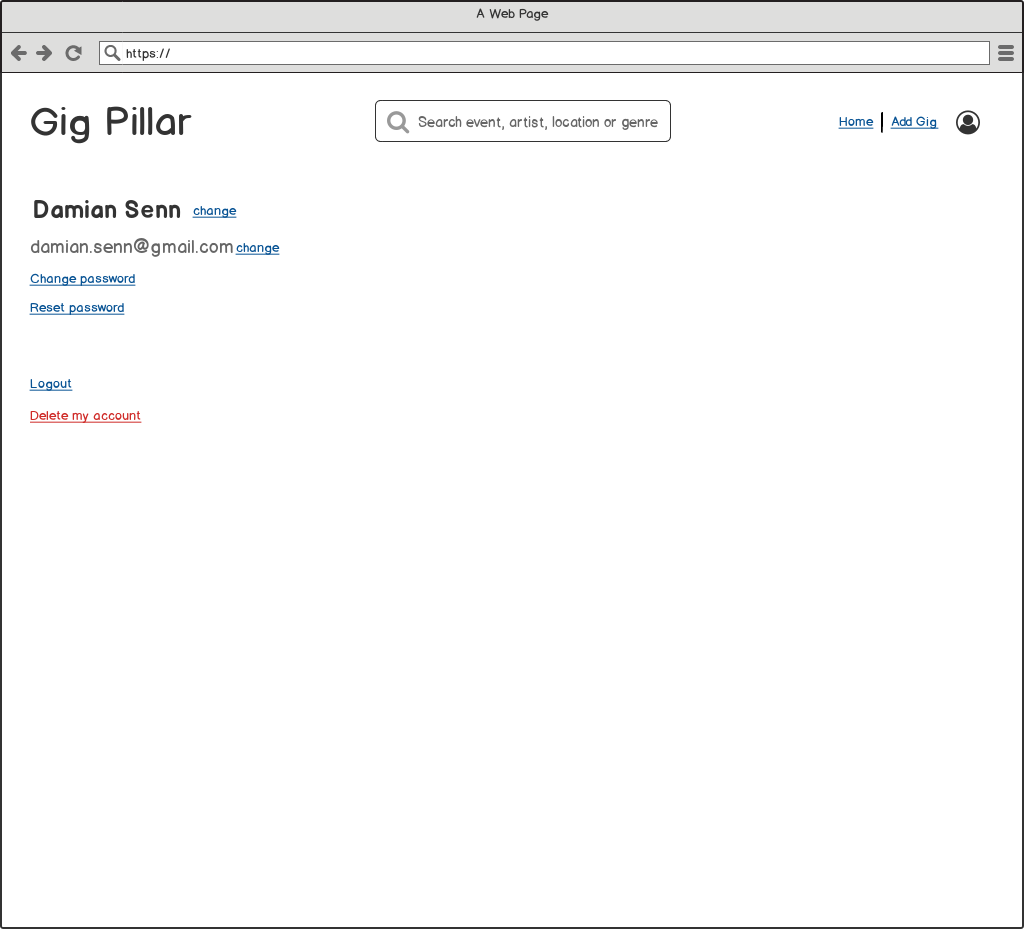
\includegraphics[width=0.95\textwidth]{mockups/profile.png}
  \caption{Mockup: Benutzerprofil}
\end{figure}

\clearpage
\section{Software}

\subsection{Datenfluss}

Die Homepage zeigt den Besuchern Gigs in ihrer Nähe an, dazu muss über eine
GeoIP API die IP-Adresse des Besuchers auf ein Land zurückverfolgt werden.
Dazu wird beim ersten Besuch die GeoIP API abgefragt und das Land des Benutzers
in eine Session geschrieben. Bei weiteren Aufrufen wird das Land direkt aus der
Session bezogen.

\begin{figure}[!htb]
  \centering
  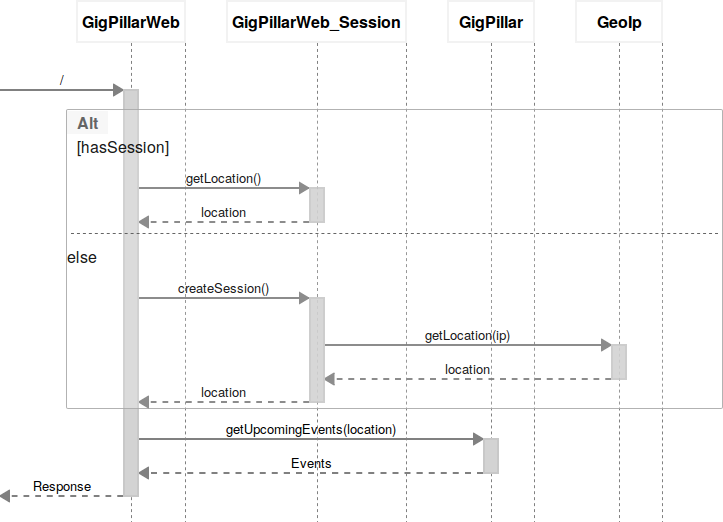
\includegraphics[width=0.95\textwidth]{konzept/datenfluss-homepage.png}
  \caption{Datenfluss: Homepage}
\end{figure}

Für weitere Datenflussdefinitionen, siehe Konzept Anhang~\ref{datenfluss}.

\clearpage
\subsection{Datenbankstruktur}

\begin{figure}[!htb]
  \centering
  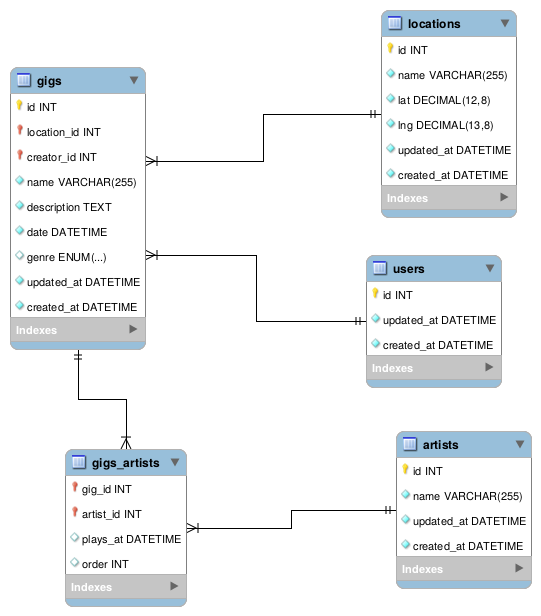
\includegraphics[width=0.95\textwidth]{konzept/erd.png}
  \caption{Konzept: Entity Relationship Diagram}
\end{figure}

\clearpage
\section{Testkonzept}

\subsection{Unit-Tests}

Der Applikationscode soll mit Unit-Tests getestet werden.

Unit-Tests testen einzelne Funktionen, d.h. hier sind Aufrufe über HTTP, wie
sie durch den Browser ausgelöst würden, oder Datenbankabfragen ausgeschlossen.

\subsection{Integration-Tests}

HTTP Requests sowie Datenabfragen sollen über Integration-Tests abgedeckt
werden. In den Integration-Tests wird vor allem Business-Logik wie z.B.
Validierungen von Daten getestet.

\subsection{Browser-Tests}

Mit der in der Studie evaluierten Testing Library «Wallaby» sollen die
gängigsten Benutzer Use-Cases getestet werden.

\subsection{Visual-Tests}

Es soll für jede Ansicht während den Tests mindestens ein Screenshot für
\href{https://percy.io/}{percy.io} erstellt werden.

\subsection{Akzeptanztests}

Die Akzeptanztest sind vom Projektleiter vor Abschluss der Realisierung
durchzuführen. Der Umfang der Akzeptanztests basiert auf den Kriterien die im
Anforderungskatalog definiert wurden.

Technische Kritierien wie die Indexierbarkeit wurden in den Akzeptanztests
bewusst ausgelassen, die Tests sollen möglichst unabhängig vom System
durchführbar sein.

Das ausführliche Testprotokoll ist im Konzept im Anhang~\ref{akzeptanztests} zu finden.

\clearpage
\section{Fazit}
\subsection{Probleme}

Für die Location Autocomplete Funktion, ist es nicht klar, ob die
Google Places API die nötigen Daten zur Verfügung stellt. So kann es gut sein,
dass Locations nicht gefunden werden oder zuviele nicht relevante Resultate
zurück gibt.

\subsection{Machbarkeit}

Für die Machbarkeit während dem im Konzept ein Test mit der Google Places API
gemacht. Die Google Places API liefert alle nötigen Daten, um die gewünschten
Features umzusetzen.

\subsection{Wirtschaftlichkeit}

In der Konzeptphase hat es keine Anzeichen auf Veränderungen, die die
Wirtschaftlichkeit beeinflussen sollte.

\subsection{Erweiterbarkeit}

Es bestehen einige Ideen, wie man die Applikation erweitern könnte. Ein Feature
wäre zum Beispiel, dass beim Erfassen eines Gigs sogleich ein Facebook-Event
angelegt würde. Weiter denkbar wäre eine Filter-Funktion, die die Gigs basierend
auf einem Radius in Kilometer um eine Stadt einschränken würde.

\subsection{Projektplan}

Trotz einer Verschiebung im Projektplans während der Initialisierung, wird nach
der Konzeptphase der Projektplan soweit eingehalten werden können. Da die
Screendesigns sowie das Testkonzept weniger Zeit beansprucht haben, bin ich
nach dem Zwischenmeeting wieder im geplanten Bereich.
